\documentclass{beamer}
\usetheme{Padova}

\title{Componente di controllo per l'elaborazione in tempo reale di flussi di dati aggregati}
\subtitle{Dipartimento di Matematica ``Tullio Levi Civita" Università di Padova, Corso di Laurea in Informatica Esame di Laurea}
\date{30 Settembre 2021}
\author{Niccolò Mantovani}



\begin{document}

	\maketitle

	\begin{frame}{Indice}
		\tableofcontents
	\end{frame}


	\section{L'azienda}

	\begin{frame}{L'azienda}

		\textbf{Datasoil s.r.l.} \vspace{.2em}
		
		\textit{Startup} Innovativa fondata nel 2016 con l'obiettivo di fare \textit{Open Innovation} nell'ambito manifatturiero. \vspace{.2em}
		
		\begin{itemize}
			\item \textit{Software as a Service} in \textit{cloud} \textbf{B2B} e \textbf{B2C} \vspace{.5em}
			\item Analisi, elaborazione e fruizione di dati \vspace{.5em}
			\item Piattaforma proprietaria \textbf{SYN}
		\end{itemize}
		
		\begin{figure}[!h] 
    		\centering 
    		
\includegraphics[width=0.2\columnwidth]{../immagini/ds_logo.png}
		\end{figure}

	\end{frame}

	\section{Il progetto}

	\begin{frame}{Il progetto}
	\vspace{.5em}
		Creazione di una componente aggiuntiva per la piattaforma \textbf{SYN} \vspace{.2em}
		
		\begin{block}{Obiettivi}
			\begin{itemize}
				\item Elaborazione \textit{streaming} di eventi provenienti da \textbf{sorgenti differenti} \vspace{.5em}
				\item Raggruppamento temporale \vspace{.5em}
				\item Raggruppamento secondo caratteristiche specifiche \vspace{.5em}
				\item Rilevazione di anomalie \vspace{.5em} 			
			\end{itemize}
		\end{block}
		
		\vspace{-0.3cm}
		\begin{figure}[!h] 
    		\centering 
    		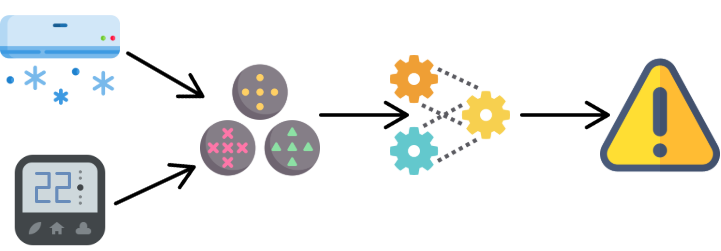
\includegraphics[width=0.55\columnwidth]{../immagini/slide/elaboration_example.png}
		\end{figure}
		
	\end{frame}
	
	\subsection{Problema affrontato}

	\begin{frame}{Problema affrontato}

		\begin{alertblock}{Adattabilità struttura dati}
			Rappresentazione di eventi facenti parte di un \textbf{gruppo} \vspace{.5em}
		\end{alertblock} \vspace{.2em}
		
		\begin{alertblock}{Adattabilità raggruppamento}
			\begin{itemize}
				\item \textbf{Temporale:} su eventi di \textbf{sorgenti differenti} \vspace{.5em}
				\item \textbf{Per caratteristiche:} su eventi di \textbf{sorgenti differenti} \vspace{.5em}
			\end{itemize}
		\end{alertblock}
		
		\begin{alertblock}{Adattabilità rilevazione anomalie}
			Rilevazione di anomalie e produzione di \textit{alert} su \textbf{gruppi} di eventi \vspace{.5em} 
		\end{alertblock}
	\end{frame}
	
	\subsection{Soluzione proposta}

	\begin{frame}{Soluzione proposta}
		\begin{exampleblock}{Adattabilità struttura dati}
			Aggiunta del campo informativo \textit{``subject"} 
		\end{exampleblock}
		
		\begin{exampleblock}{Adattabilità raggruppamento}
			\begin{itemize}
				\item \textbf{Temporale:} aggregazione o allineamento tramite \textbf{configurazione}\vspace{.5em}
				\item \textbf{Per caratteristiche:} filtraggio definito dalla \textbf{configurazione}  \vspace{.5em}
			\end{itemize}
		\end{exampleblock}
		
		\begin{exampleblock}{Adattabilità rilevazione anomalie}
			Creazione di un evento riassuntivo
		\end{exampleblock}
	\end{frame}
	
	\section{Strumenti utilizzati}

	\begin{frame}{Strumenti utilizzati}
		\begin{block}{Framework}
			\begin{itemize}
				\item \textbf{Apache Flink:} \textit{data processing} per l'elaborazione di dati in modo distribuito \vspace{.5em}
				\item \textbf{ScalaTest:} stesura dei test relativi all'analisi effettuata da \textit{Flink} \vspace{.5em}
			\end{itemize}
		\end{block}
		
		\begin{block}{Linguaggi di programmazione}
			\begin{itemize}
				\item \textbf{Scala:} utilizzato tramite \textit{Flink} \vspace{.5em}
				\item \textbf{Go:} utilizzato per le \textit{API} \vspace{.5em}
			\end{itemize}
		\end{block}
	\end{frame}
	
	\subsection{Apache Flink}
	\begin{frame}{Apache Flink}
		\begin{figure}[!h] 
    		\centering 
    		
\includegraphics[width=0.27\columnwidth]{../immagini/slide/Apache_Flink_logo.png}
		\end{figure}
		
		\begin{itemize}
			\item \textbf{DataStream}
				\begin{figure}[!h] 
    		\centering 
    		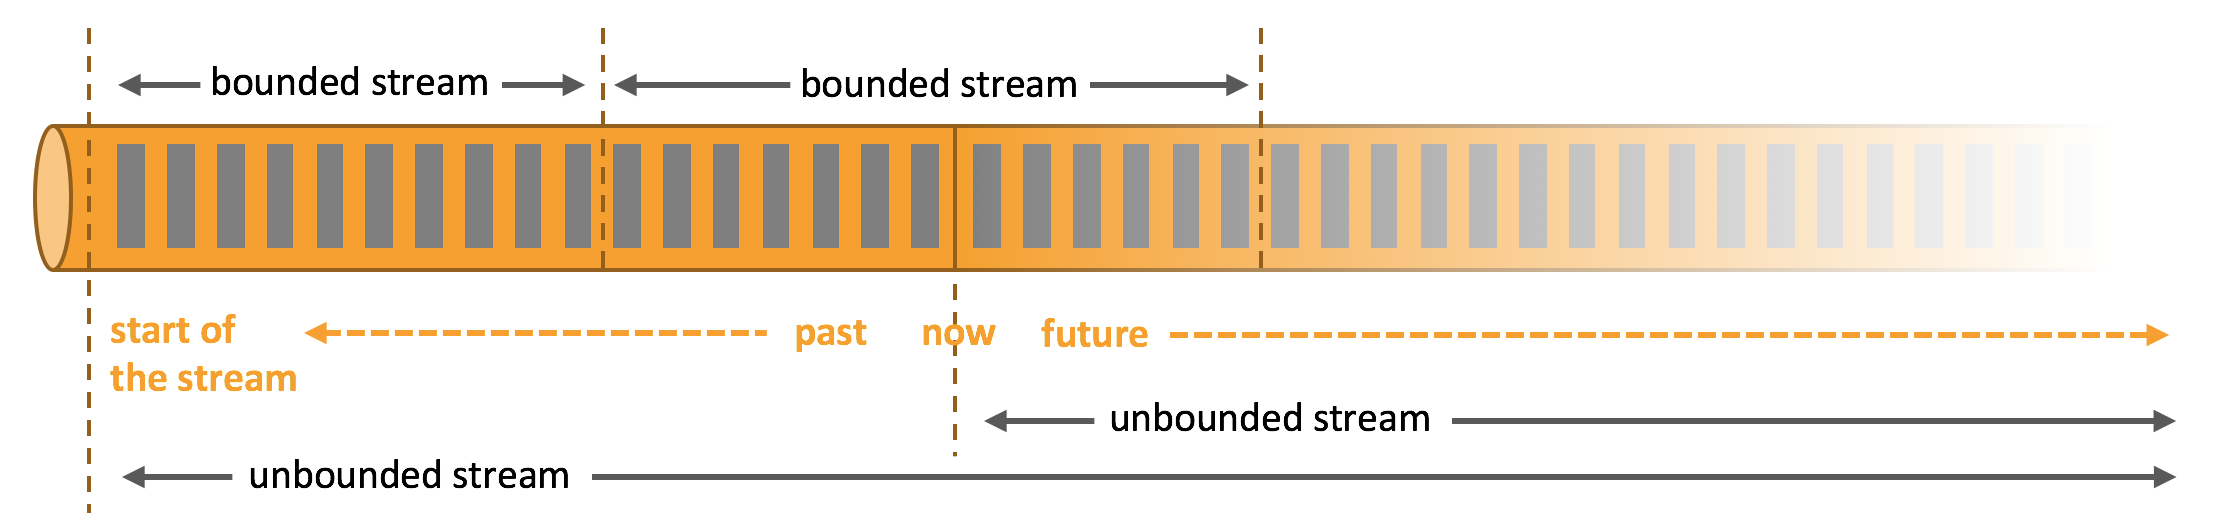
\includegraphics[width=0.8\columnwidth]{../immagini/slide/bounded-unbounded.png} 
		\end{figure}  \vspace{.5em}
			
			\item \textbf{Operatori}  \vspace{.5em}
			\item \textbf{Alta disponibilità e recovery} \vspace{.2em}
			\begin{itemize}
				\item \textit{Checkpoint} \vspace{.5em}
				\item \textit{Savepoint} \vspace{.5em}
				\end{itemize} \vspace{.5em}
		\end{itemize}
	\end{frame}
	
	\begin{frame}{Apache Flink}
		\textbf{Scalabilità}
		\vspace{.2em}
		\begin{figure}[htb]
			%\hspace{-2em}
    			\begin{minipage}[t]{0.45\textwidth}
    			
       		\centering 
    			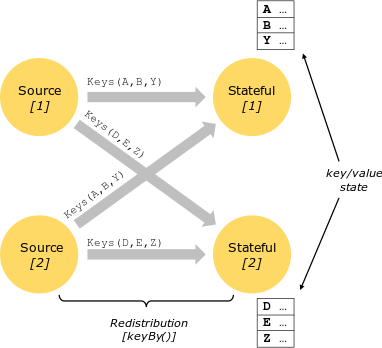
\includegraphics[width=1\columnwidth]{../immagini/tecnologieUtilizzate/flink/state_partitioning.png}
    			\end{minipage}
    			\hfill
    			\begin{minipage}[t]{0.45\textwidth}
    				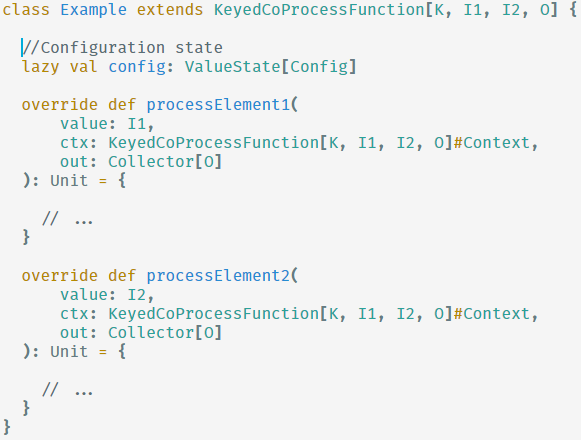
\includegraphics[width=1.25\columnwidth]{../immagini/slide/pfExample.png}
       		\end{minipage}
       		\hspace{1em}
		\end{figure}		
	\end{frame}
	
	\section{Implementazione}

	\begin{frame}{Implementazione}
		\begin{figure}[!h]
    		 \centering
    		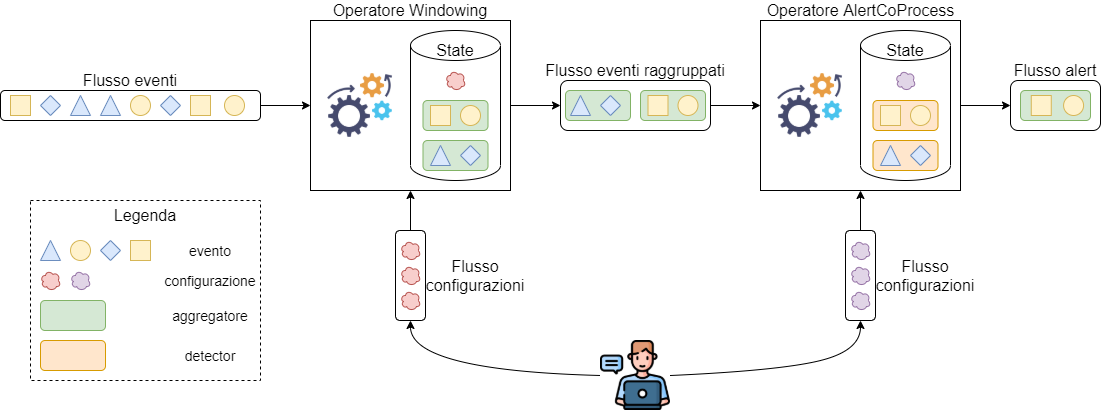
\includegraphics[width=11.5cm]{../immagini/slide/implementation.png}
		\end{figure}
	\end{frame}
	
	
	
	\section{Prodotto finale}

	\begin{frame}{Prodotto finale}
		La componente soddisfa i seguenti \textbf{requisiti}:
		\vspace{.2em}
		\begin{itemize}
			\item Analisi di eventi relativi ad \textit{asset} differenti raggruppati \vspace{.5em}
			\item Emissione di \textit{alert} \vspace{.5em}
			\item Modifica della configurazione \textit{``a caldo"} \vspace{.5em}
			\item Mantenimento analisi relativo ad \textit{asset} singoli \vspace{.5em}
			\item \textit{API} per il controllo dei dati di configurazione \vspace{.5em}
			\item Test di \textit{API} e operatori di \textit{Flink} \vspace{.5em}
		\end{itemize}
	\end{frame}
	
	\section{Considerazioni}

	\begin{frame}{Considerazioni}
		\begin{block}{Obiettivi formativi}
			\begin{itemize}
				\item \textbf{Minimi:}
					\begin{itemize}
						\item comprensione \textit{workflow} aziendale \vspace{.5em}
						\item comprensione linguaggi e architetture \vspace{.5em}
						\item definizione architettura componente \textit{anomaly detection} \vspace{.5em}
						\item definizione \textit{API} di governo \vspace{.5em}
					\end{itemize}
			\end{itemize}
		\end{block}
		
		\begin{figure}[!h]
    		 \centering
    		
\includegraphics[width=1.7cm]{../immagini/slide/100-percent.png}
		\end{figure}
	\end{frame}
	
	\begin{frame}{Considerazioni}
		\begin{block}{Obiettivi produttivi}
			\begin{itemize}
				\item \textbf{Minimi:} 
					\begin{itemize}
						\item completamento operatore \textit{Windowing} \vspace{.5em}
						\item completamento operatore \textit{AlertCoProcess} \vspace{.5em}
						\item completamento \textit{API} di governo \vspace{.5em}
					\end{itemize}
				\item \textbf{Massimi:}
					\begin{itemize}
						\item Test automatizzati operatori \textit{Flink} \vspace{.5em}
						\item Test automatizzati \textit{API} \vspace{.5em}
					\end{itemize}
			\end{itemize}
		\end{block}
		
		\begin{figure}[!h]
    		 \centering
    		
\includegraphics[width=1.7cm]{../immagini/slide/100-percent.png}
		\end{figure}
	\end{frame}
	
	\begin{frame}{Considerazioni}
		\begin{block}{Possibili miglioramenti ed estensioni}
			\begin{itemize}
				\item \textbf{Nuovi detector:} 
					\begin{itemize}
						\item \textit{Unsupervised}: rilevazione delle anomalie a livello di gruppo \vspace{.5em}
						\item \textit{UDF (User Defined Function)}: basato su \textbf{regole} decise dall'utente \vspace{.5em}
					\end{itemize}
			\end{itemize}
		\end{block}
		
		\begin{figure}[!h]
    		 \centering
    		
\includegraphics[width=1.7cm]{../immagini/slide/increasing-bar-graph.png}
		\end{figure}
	\end{frame}
	
	\subsection{Conoscenze acquisite}

	\begin{frame}{Conoscenze acquisite}
		\begin{figure}[!h]
    		 \centering
    		
\includegraphics[width=1\columnwidth]{../immagini/slide/learned.pdf}
		\end{figure}
	\end{frame}


\end{document}
